\documentclass[11pt]{article}
\usepackage{amsmath,amsthm,amsfonts,amssymb}
\usepackage[normalem]{ulem}
\usepackage{graphicx}
\usepackage{float}
\usepackage{hyperref}
\usepackage{comment}



\newtheorem{theorem}{Theorem}
\newtheorem{lemma}{Lemma}
\newtheorem{corollary}{Corollary}
\newtheorem{proposition}{Proposition}
\theoremstyle{definition}
\newtheorem{definition}{Definition}
\theoremstyle{basic}


\newcommand{\N}{\mathbb{N}}
\newcommand{\R}{\mathbb{R}}
\newcommand{\AVG}{\mathrm{AVG}}
\newcommand{\VAR}{\mathrm{VAR}}
\newcommand{\STDDEV}{\mathrm{STDDEV}}
\newcommand{\calX}{\mathcal{X}}
\newcommand{\calD}{\mathcal{D}}



\title{CS 886 Project Proposal\\Modeling Effects of Social Relationship in Opinion Dynamics}
\author{Haotian Zhang\\Advisor: Robin Cohen\\University of Waterloo\\h435zhan@uwaterloo.ca}
\date{}


\begin{document}
\maketitle

\begin{abstract}
The opinions of social media users are greatly shaped and influenced
by their social network friends (neighbors). Understanding how users
iteratively update opinions based on opinions from their neighbors 
is critical in the context of modeling opinion formation and informational influence for social network research.
We find that existing and widely studied opinion dynamics models
consider the neighbors of a certain agent dynamically change their opinions according to the similarity. And these models would
be more receptive to agents with higher homophily
or more similar opinions while becoming more skeptical of others. However, this assumption ignores the fact that most users maintain a relatively stable acquaintance
network with some of their close family members or friends. And degrees of friendship with different types of neighbors could affect agents' opinions to varying extent. In this
paper, we propose a novel model which takes the degree of friendship as 
a variable into consideration. Via controlled experiments,
we want to find out the how user update opinions based on opinions from
neighbors with varying friendship degree.

\end{abstract}

\section{Introduction}

\section{Related Work}
\cite{tsang2014opinion} Skepticism model explore the effects of skepticism between agents.

\section{Acquaintance Opinion Dynamics Model}
Based on DEGROOT model \cite{das2014modeling} and skepticism model \cite{tsang2014opinion}, we propose a new model that combines the variance of friendship with traditional averaging model. Agents $\{1,2,...,n\}$ are connected by Erd\"{o}s R\'{e}nyi random graph $G=(V,E)$. $x_i \in [0,1]$ represents the opinion held by agent $i$. For each agent, $i$ has two sets of adjacent edges $E_O$ and $E_C$ which stand for the connections with close friends and ordinary neighbors respectively. In other words, agent $i$ has two types of neighbors close fridens: $C(i)=\{v \in V|\{i,v\}\in E_C\}$; and ordinary neighbors: $O(i)=\{v \in V|\{i,v\}\in E_O\}$ with different acquaintance degree. 

In this model, agent $i$ is parameterized by one innate quantity: $\alpha$ is termed as the \textbf{acquaint parameter} to measure the probability to be persuaded by someone with closer relationship. We hypothesis that agent's opinion is more likely to be affected by his family members and close friends. Other types of neighbors can not achieve the same level of influence.
The opinion $x_i$ is also influenced by various types of neighbors with different trust values: $y_{i,j}>0$ for close friends and $w_{i,k}>0$ for ordinary neighbors. There also exists a weight $w_{i,i}$ contributed to the agent's innate opinion. We assume $w_{i,i}>c\times\sum_{k\in{O_i}}w_{i,k}$.

\begin{equation}
x_i \gets \frac{w_{i,i}x_i + \alpha\sum\limits_{j \in C(i)}y_{i,j}x_j + (1-\alpha)\sum\limits_{k \in O(i)}w_{i,k}x_k}{w_{i,i}x_i + \alpha\sum\limits_{j \in C(i)}y_{i,j} + (1-\alpha)\sum\limits_{k \in O(i)}w_{i,k}}
\end{equation} 

\begin{equation}
w_{i,k} \gets \frac{w_{i,k} + rT(x_i,x_k)}{1+r}
\label{ordinary.weight}
\end{equation}

In this model, we assume $\min\limits_{{j}\in C_i}{y_{i,j}} > \max\limits_{{k}\in O_i}{w_{i,k}}$ since that the agent $i$ remains more receptive to his acquaintances $C_i$ than other ordinary neighbors $O_i$ in most cases. As indicated in Equation \ref{ordinary.weight}, for $w_{i,k}$ updated in each iteration, it is updated via trust function $T$ which is based on distance between opinions $x$ and $x{'}$ via the Gaussian kernel shown in Equation \ref{trust}. $r$ is defined as the learning rate of the population; higher $r$ means the agent would distrust other agents with different opinion more quickly. And it would lead to faster generation of small group which only hold similar opinions.

\begin{equation}
T(x,x{'})=exp(-\frac{(x-x{'})^2}{h})
\label{trust}
\end{equation} 

$h$ is the empathy of the population: a higher $h$ means agents are more easily influenced by other agents with different opinions. The trust value $y_{i,j}$ is assigned to $i$'s closer acquaintance. We assume the degree distribution of acquaintance networks follows a power-law distribution \cite{muchnik2013origins}. So only limited neighbors can be regarded as acquaintances in our defined model. Currently, we set all weights as $\{y_{i,j}=1|j \in C_i\}$ to simplify the simulation process. 

\begin{comment}
\section{Background and Related Work}

Sentiment analysis is a hot and well-studied topic in NLP. One simple model for sentiment analysis is the bag-of-words model, which vectorizes a paragraph or sentences as the occurrence counts for each word, and this model can also combine with the tf-idf measure to extract keywords from texts.
However, the bag-of-words model cannot capture the order of words in the text or the structure information of sentences\cite{pennington2011semi}.

\subsection{Word Embedding}

It seems that word embedding is one of the most interesting topic in deep learning at the moment.
In fact, word embedding was originally introduced by Bengio et al.\ in 2001.
A word embedding $W : w\rightarrow \mathbb{R}^k$ is a function mapping words of the language into $k$-dimensional vectors, called \textit{word vector}.
The word vectors can put similar words close together in the vector space, which captures some syntactic and semantic information between words.
For example, $d(\mbox{China}, \mbox{Beijing}) \approx d(\mbox{Canada}, \mbox{Ottawa})$, $d(\mbox{Microsoft}, \mbox{Windows}) \approx d(\mbox{Google}, \mbox{Android})$.
And the word vectors can be trained by skip-gram or continuous bag-of-words model in an unsupervised way. 


\subsection{Convolutional Neural Network}

Convolutional neural networks (CNN) utilize layers with convolving filters that are applied to local features\cite{lecun1995convolutional}.
CNN was originally invented for computer vision, but recently lots of studies show that CNN models have subsequently been effective for NLP tasks and have achieved excellent results in semantic parsing, search query retrieval, sentence modeling, and other NLP tasks.
Some state-of-the-art results of sentiment analysis or other NLP tasks come from convolutional neural network.
In 2014, all Kim, Kalchbrenner et al.\ and Cicero et al.\ use convolutional neural networks for different sentiment analysis tasks and get better results than previous ones.


Kalchbrenner et al.\cite{kalchbrenner2014convolutional}\ describe a dynamic CNN that uses the dynamic $k$-max pooling operator as a non-linear sub-sampling function.
Their experiments show that this model can achieve good accuracy without requiring external features or other resources.
%48.5% 86.8%


Kim\cite{kim2014convolutional} proposes a simple CNN using a single convolutional layer and max-pooling layer to achieve a similar result.
In his paper, he introduces multi-channel word vectors as the input of CNN, and uses both static and non-static pre-trained word vectors with the intermediate feature map being the sum of the two resulting feature maps.
The static pre-trained word vectors are trained by Mikolov et al.\ on 100 billion words of Google News\cite{DBLP:journals/corr/abs-1301-3781, DBLP:journals/corr/MikolovSCCD13}.

%He also empirically shows that with his multi-channel model, he achieves 47.4\% accuracy on the 5-label movie review sentiment classification task (the SST-1 dataset) and 88.1\% on the binary classification task(the SST-2 dataset).


Cicero et al.\cite{dos2014deep}\ introduce CharSCNN which combines word-level embeddings with character-level embeddings as the input of CNN to extract a sentence-level representation. 
Both character-level embeddings and word-level embeddings are trained during network training phase.
They also demonstrate that a feed-forward neural network architecture can be as effective as RNTN for sentiment analysis of sentences.
%They also show that they achieve 48.3\% accuracy on the SST-1 dataset and 85.7\% accuracy on the SST-2 dataset.


%All of these 3 papers 

\section{Approach}

My work is based on Kim's convolutional neural network with many modifications.
The model architecture is a multi-layer convolutional neural network.

Suppose we have a review of length $n$, $X = \{x_1, x_2, \ldots, x_n\}$, where $x_i \in \mathbb{R}^K$ is the $K$-dimensional word vector corresponding to the $i$-th word in the sentence.
Here, $X$ is the input of the CNN.

\subsection{Convolutional Layers}

In this model, we have 2 convolutional layers with the same number of filters $F$, but they have different window size $h_1, h_2$.

For the first convolutional layer, it involves $F$ filters $w \in \mathbb{R}^{h_1K}$, which are applied to a window of $h_1$ words to produce a new feature, i.e.\ a feature $c_i$ is generated from a window of words $x_i,\ldots, x_{i + h_1 - 1}$ by $c_i = f(w \cdot [x_i \ldots x_{i + h_1 - 1}] + b)$.
Here, $f$ is an activation function such as \textit{rectified linear unit (ReLU)}, \textit{sigmoid} or \textit{hyperbolic tangent ($\tanh$)}, and $b$ is a bias term.
So the output of the first convolutional layer for each filter is a feature map $c = [c_1, c_2, \ldots, c_{n - h_1 + 1}] \in \mathbb{R}^{n - h_1 + 1}$.
I then appy a variant max-over-time pooling operation, which takes the maximum value over every two elements, i.e.\ $maxpool(c) = [\max\{c_1, c_2\}, \max\{c_3, c_4\}, \ldots, \max\{n - h_1, n - h_1 + 1\}]$, and $maxpool(c)$ is the input of the next convolutional layer.

The second convolutional layer is similar to the first with the following differences,
\begin{itemize}
    \item the window size changes to $h_2$ and the input is a vector for each previous layer filter, so the filters changes to $w' \in \mathbb{R}^{h_2}$
    \item apply the conventional max pooling operation, which takes the maximum over the feature map, i.e.\ $maxpool'(c') = \max\{c'_i\}$
\end{itemize}
So after two convolutional layer, the output is a new feature map $C = [C_1, \ldots, C_F]$ over all $F$ filters. I also add some dropout operations in this architecture to prevent feature co-adaption.


\subsection{Fully-connected Layers}

In this phase, I add 3 hidden fully-connected layers to extract the features among the feature map generated from previous layers.
This can also be thought as a dimensionality reduction process.
Our input dimension is $F$, and the output depends on whether the label is binary or categorical; if it is binary, the output is $\{0,1\}$, otherwise it is $\{0,1\}^{\left|label\right|}$, which is a bit vector of the size of labels.

\begin{itemize}
    \item the first hidden layer is a mapping function $\mathbb{R}^F \rightarrow \mathbb{R}^{D_1}$,
    \item the second hidden layer, connected to the first one, is also a mapping function $\mathbb{R}^{D_1} \rightarrow \mathbb{R}^{D_2}$,
    \item and the last hidden layer outputs the final label, $\mathbb{R}^{D_2} \rightarrow \{0,1\}\mbox{ or }\{0,1\}^{\left|label\right|}$
\end{itemize}

Here, the $D_1, D_2$ are the parameters chosen in the next section.



\section{Experiments}

\subsection{Yelp Review Datasets}

I use the Yelp Academic dataset, which consists of 1.6M reviews and 500K tips by 366K users for 61K businesses, and all of the dataset are in the JSON file format.
For each of reviews, it contains several fields, such as business id, user id, stars, text, date and votes.
In this project, I only use \textit{text} field, which is a natural language text, and \textit{stars} field, which is an integer rating for that review.


\begin{table}
\centering
\begin{tabular}{c|c|c|c|c|c}
Stars & 1 & 2 & 3 & 4 & 5\\\hline
Percentage & 10.18\% & 8.96\% & 14.19\% & 29.73\% & 36.93\%
\end{tabular}
\caption{Distribution of star ratings}
\label{table0}
\end{table}

The longest review involves 1047 words, 4963 characters among all reviews, and the average sentence length is 125.38 words.
Table \ref{table0} gives the distribution over star ratings.
It shows that Yelp dataset if highly skewed toward positive ratings.


\subsection{Preprocessing}

Actually, the Yelp text reviews is really a dirty corpus, since it contains many inform English words, punctuations, even Emojis.
To clean the corpus, I throw away all the special symbols and punctuations and convert all English letters into lowercase.
But exceptions do exist.
For some special cases, I use the underscore symbol (\_) to link words.
For example,
\begin{itemize}
    \item ``China'' $\rightarrow$ ``china''
    \item ``part-time'' $\rightarrow$ ``part\_time''
    \item ``Let's'' $\rightarrow$ ``let\_s''
    \item ``Tasty! \^\_\^\ '' $\rightarrow$ ``tasty''
\end{itemize}

As I discussed above, the rating stars given by users cannot be objective, and from analysis of the dataset, I found that the average rating is 3.743 stars.
Many of the most ambiguous reviews are focus on 3 stars.
Therefore, I finally decide to drop out all the reviews with 3 stars to make the dataset more objective.
To make things more extreme, I also do some experiments on the binary classification,
\begin{itemize}
    \item mapping 1 star and 2 stars to Negative, mapping 4 stars and 5 stars to Positive
    \item only use 1 star and 5 stars reviews, and make 1 star as Negative and make 5 stars as Positive
\end{itemize}
Obviously, the accuracy of binary classification is much better than multi-class classification as we would discuss later.

Another problem from corpus is the various length of review texts.
To fix this issue, I only use the reviews which involve number of words less than or equal 150, which is approximately equal the average length of reviews in the dataset.
If the length of some reviews cannot reach 150, I add padding zero vectors at the end to fix the length of review text.

\subsection{Training Word Vectors}

I use the tools \textit{word2vec} (Mikolov et al.\ 2013) to pre-train the word vectors.
Instead of using Google News as training corpus, I prefer use native Yelp review texts.
One of important reasons is Yelp reviews consist of many informal and casual words and phrases, so if I use Google News which is much more formal, I may lose many useful information in the text.

Another issue is how to choose the dimension $K$ of the word vectors.
I empirically tried $K = 50$ and $K = 150$, and the results show that the difference between them is negligible.
Therefore, I finally consider the data scale, and choose $K = 50$ as the dimension of the word vectors.

Here, I list some of the similar words given by the word vectors (ranked by distance),

\begin{itemize}
    \item chinese - asian, vietnamese, korean, cantonese, japanese
    \item tofu - rice, noodles, kimchi, eggplant, vegetable
    \item tomato - tomatoes, pesto, avocado, cheese, mushroom, onions
    \item yummy - delish, delicious, tasty, yum, scrumptious, yummm, mmmm (some informal words)
    \item bbq - barbecue, barbeque, brisket, ribs, kalbi
    \item apple - apples, pecan, peach, apricot, blackberry, blueberry
\end{itemize}

The word vectors really capture much syntactic and semantic information from corpus.

\subsection{Environment Settings}

I implemented the aforementioned multi-layer CNN using Keras, an open source CNN library based on Python and C and support CUDA GPU acceleration.
The specification of my machine is 16GB main memory and Nvidia Geforce GTX 750 Ti graphics card (2GB graphics card memory, 640 cores).
After I preprocess the dataset and embed word vectors, the training data become extremely large.
Because of the limitation of my machine's memory and GPU, I could only use at most 3\% data, which approximately involves 50K reviews. 
Nevertheless, I still achieve high accuracy by this model.

All values of parameters I used in CNN are listed here,

\begin{itemize}
    \item Dimension of word vectors, $K = 50$
    \item Length of review text, $n = 150$
    \item Number of filters applied in convolutional layers, $F = 128$
    \item Window size of filters, $h_1 = 3, h_2 = 5$
    \item Dimension of hidden fully-connected layers, $D_1 = 64, D_2 = 8$
    \item Number of epochs during training and optimizing, $E = 5$
\end{itemize}

\subsection{Result}

\begin{table}
\centering
\resizebox{\linewidth}{!}{%
\begin{tabular}{c|c|c|c|c|c|c|c|c|c|c|c}
\#reviews & 1030 & 4919 & 9864 & 14691 & 19426 & 24271 & 29238 & 33979 & 39013 & 43692 & 48843\\\hline
ratio\% & 0.1 & 0.5 & 1.0 & 1.5 & 2.0 & 2.5 & 3.0 & 3.5 & 4.0 & 4.5 & 5.0\\\hline
accuracy\% & 81.38 & 91.76 & 92.71 & 93.14 & 93.34 & 93.36 & 93.26 & 94.09 & 92.81 & 94.09 & 94.05
\end{tabular}%
}
\caption{Accuracy - training size of binary classification on reviews with 1, 2, 4, 5 stars}
\label{tableA}
\end{table}

\begin{table}
\centering
\resizebox{\linewidth}{!}{%
\begin{tabular}{c|c|c|c|c|c|c|c|c|c|c|c}
\#reviews & 586 & 2864 & 5569 & 8379 & 11247 & 13908 & 16949 & 19684 & 22554 & 25113 & 28130\\\hline
ratio\% & 0.1 & 0.5 & 1.0 & 1.5 & 2.0 & 2.5 & 3.0 & 3.5 & 4.0 & 4.5 & 5.0\\\hline
accuracy\% & 81.41 & 93.83 & 94.84 & 95.65 & 95.56 & 95.61 & 95.84 & 96.20 & 96.25 & 96.38 & 96.56\\\hline\hline
\#reviews & 30739 & 33374 & 36288 & 38625 & 42171 & 44768 & & & & & \\\hline
ratio\% & 5.5 & 6.0 & 6.5 & 7.0 & 7.5 & 8.0 & &  &  &  & \\\hline
accuracy\% & 96.47 & 96.75 & 96.65 & 96.70 & 96.16 & 96.79 & & & & & 
\end{tabular}%
}
\caption{Accuracy - training size of binary classification on reviews with only 1, 5 stars}
\label{tableB}
\end{table}


\begin{table}
\centering
\resizebox{\linewidth}{!}{%
\begin{tabular}{c|c|c|c|c|c|c|c|c|c|c|c}
\#reviews & 1001 & 4777 & 9797 & 14570 & 19678 & 26539 & 29348 & 33920 & 39272 & 44234 & 49004\\\hline
ratio\% & 0.1 & 0.5 & 1.0 & 1.5 & 2.0 & 2.5 & 3.0 & 3.5 & 4.0 & 4.5 & 5.0\\\hline
accuracy\% & 45.35 & 56.42 & 64.94 & 65.00 & 62.76 & 66.53 & 66.31 & 65.83 & 64.43 & 65.68 & 66.61
\end{tabular}%
}
\caption{Accuracy - training size of multi-class classification on reviews with 1, 2, 4, 5 stars}
\label{tableC}
\end{table}

\begin{figure}
\centering
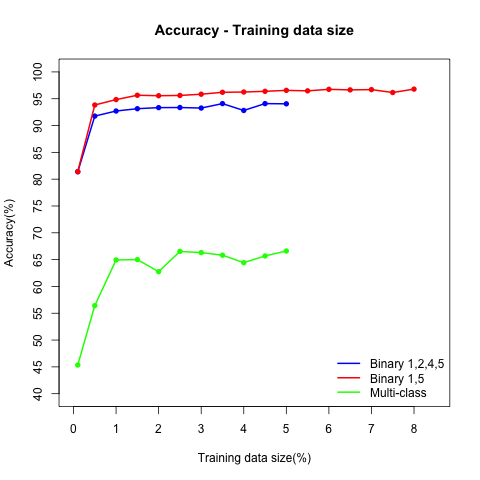
\includegraphics[scale=0.6]{figure.png}
\caption{Accuracy - Training data size}
\label{figureA}
\end{figure}


For binary classification with 1, 2, 4, 5 stars, shown in Table \ref{tableA} and Figure \ref{figureA}, the highest accuracy achieve 94.09\%.
The testing set contains 4926 reviews (0.5\%).

For binary classification with 1, 5 stars, shown in Table \ref{tableB} and Figure \ref{figureA}, the highest accuracy achieve 96.79\%.
The testing set contains 5606 reviews (1.0\%)

For multi-class classification with 1, 2, 4, 5 stars, shown in Table \ref{tableC} and Figure \ref{figureA}, the highest accuracy achieve 66.61\%.
The testing set contains 4732 reviews (0.5\%).

Yu and Chang\cite{Yu} use recurrent neural network (RNN) with long short-term memory (LSTM) and an one-layer CNN to give several previous results on the same dataset for multi-class classification.
Table \ref{tableD} shows the model comparison.

\begin{table}
\centering
\begin{tabular}{c|c}
Model & Accuracy\\\hline
Multi-layer CNN & 0.66\\\hline
Softmax regression & 0.45\\
RNN with LSTM & 0.51\\
CNN with zero padding & 0.32\\
CNN with chunking & 0.34
\end{tabular}
\caption{Model Comparison - Multi-class Classification}
\label{tableD}
\end{table}

For binary classification task on Yelp review dataset, Jong\cite{Jong} shows some results from other possible models.
Table \ref{tableE} shows the model comparison.

\begin{table}
\centering
\begin{tabular}{c|c}
Model & Accuracy\\\hline
Multi-layer CNN & 0.94\\\hline
Naive Bayes & 0.78\\
SVM & 0.74\\
Word Vector + SVM & 0.69
\end{tabular}
\caption{Model Comparison - Binary Classification}
\label{tableE}
\end{table}

\paragraph{Remark}
Though my result is much better than previous results, there exists some factors in my experiments which make the result good.
First, I drop all reviews with 3 stars rating, which are the most ambiguous for learning models.
Second, I drop all the long reviews, which can involve some complex logic relation and context and hard to learn.
Third, I use Yelp review dataset to pre-train word vectors instead of Google News, which probably can capture more information from text.

\section{Conclusion and Future Work}

This work should be the first multi-layer CNN model using word embedding on the Yelp review dataset.
Currently, I just try 2-layer architecture and only use the word vectors as the input feature.
And I have though several possible extensions and future works which I could try.

\begin{itemize}
    \item \textbf{Visualization}
    In this project, the multi-layer CNN model is implemented using Keras.
    However, Keras does not provide a good visualization API to inspect the features learned by each neural.
    This could a barrier if we expect to design a better multi-layer CNN and improve the result. 
    \item \textbf{Size of Dataset}
    As I mentioned, I can only use at most 3\% data because of limit computation resource of my machine and inherent ambiguity of the dataset.
    If I could use more dataset, we definitely can improve the accuracy.
    \item \textbf{CNN architecture and Features}
    It is possible to add more language model features as the input of CNN combing with the powerful word embedding.
    Also, it is possible to make the neural network deeper and deeper to extract implicit features for sentiment analysis.
    \item \textbf{Other NLP tasks}
    I could also use this model try for other NLP tasks.
\end{itemize}

\subsection*{Acknowledgments}

I would like to thank Haotian Zhang, Siwei Yang, Yahui Chen and Hisham El-Zein for their suggestions and discussions.
\end{comment}

\bibliography{report}
\bibliographystyle{plain}


\end{document}  